\chapterimage{chapter_8.png}
\chapter{图论}
\begin{center}
    \pgfornament[width=0.36\linewidth,color=lsp]{88}
\end{center}

\section{二分图}
二分图常用来判断是否能分成两组

\subsection{检测二分图}
\lstinputlisting[style=cpp]{code/graph/isbipartition.cpp}

\ifshowLink
相关题目:
    \begin{enumerate}
        \item LeetCode 886. Possible Bipartition: \href{https://leetcode.cn/problems/possible-bipartition/}{https://leetcode.cn/problems/possible-bipartition/}
    \end{enumerate}
\fi

\section{拓扑排序}
对于图论,直观来说,就是把一副图\textbf{拉平},而且在这个拉平的图里,所有箭头方向都是一致的。

\begin{figure}[H] %H为当前位置,!htb为忽略美学标准,htbp为浮动图形
\centering %图片居中
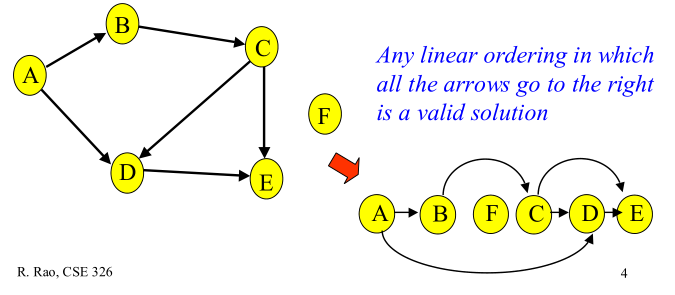
\includegraphics[width=0.7\textwidth]{images_content/0.png} %插入图片,[]中设置图片大小,{}中是图片文件名
\caption{Topological Sorting} %最终文档中希望显示的图片标题
\end{figure}
1. 对于\textbf{DFS}, 将后序遍历的结果进行反转,就是拓扑排序的结果

2. 对于\textbf{BFS} (也就是\textbf{kahn算法}), 参考代码如下:
\lstinputlisting[style=cpp]{code/graph/topological_sorting.cpp}

\ifshowLink
相关题目:
    \begin{enumerate}
        \item LeetCode 210. Course Schedule II: \href{https://leetcode.cn/problems/course-schedule-ii/}{https://leetcode.cn/problems/course-schedule-ii/}
    \end{enumerate}
\fi